\begin{figure}
	\centering
	\begin{subfigure}[b]{0.2\textwidth}
		\centering
		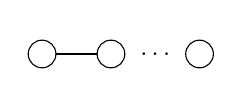
\begin{tikzpicture}[
			wide/.style={line width=4pt}, every node/.style={circle,draw,minimum size=10}, scale=.25]

			\node (root) at (-3.5,0) {};
			\node (child) at (0,0) {};
			\node (end) at (4.5,0) {};

			\draw (root) -- (child);
			\path (child) -- (end) node[midway, draw=none,fill=none] {\small $\dots$};

		\end{tikzpicture}
		\subcaption{}\label{subfig:multistage-pandora}
	\end{subfigure}
	\hfil
	\begin{subfigure}[b]{0.2\textwidth}
		\centering
		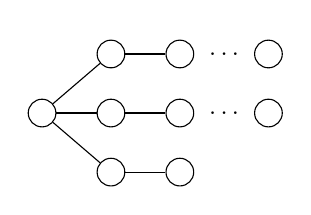
\begin{tikzpicture}[
			wide/.style={line width=4pt}, every node/.style={circle,draw,minimum size=10}, scale=.25]

			\node (root) at (-7, 0) {};

			\node (s1) at (-3.5,3) {};
			\node (s2) at (0,3) {};
			\node (s3) at (4.5,3) {};

			\draw (s1) -- (s2);
			\path (s2) -- (s3) node[midway, draw=none,fill=none] {\small $\dots$};

			\node (s4) at (-3.5,0) {};
			\node (s5) at (0,0) {};
			\node (s6) at (4.5,0) {};

			\draw (s4) -- (s5);
			\path (s5) -- (s6) node[midway, draw=none,fill=none] {\small $\dots$};

			\node (s7) at (-3.5,-3) {};
			\node (s8) at (0,-3) {};

			\draw (s7) -- (s8);

			\draw (root) -- (s1);
			\draw (root) -- (s4);
			\draw (root) -- (s7);
		\end{tikzpicture}
		\subcaption{}\label{subfig:cabinets}
	\end{subfigure}
	\hfil
	\begin{subfigure}[b]{0.2\textwidth}
		\centering
		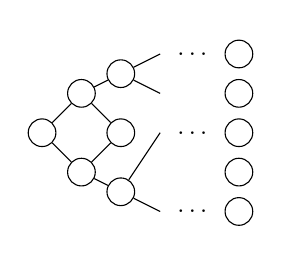
\begin{tikzpicture}[
			wide/.style={line width=4pt}, every node/.style={circle,draw,minimum size=10}, scale=.25]

			\node (root) at (-4,0) {};

			\node (s1) at (-2, 2) {};
			\node (s2) at (-2, -2) {};

			\node  (s3) at (0, 3) {};
			\node  (s4) at (0, 0) {};
			\node  (s5) at (0, -3) {};

			\coordinate  (s6) at (2, 4) {};
			\coordinate  (s7) at (2, 2) {};
			\coordinate  (s8) at (2, 0) {};
			\coordinate  (s9) at (2,-4) {};

			\node (b1) at (6, 4) {};
			\node (b2) at (6, 2) {};
			\node (b3) at (6, 0) {};
			\node (b4) at (6, -2) {};
			\node (b5) at (6, -4) {};

			\draw (root) -- (s1);
			\draw (root) -- (s2);

			\draw (s1) -- (s3);
			\draw  (s1) -- (s4);

			\draw  (s2) -- (s4);
			\draw  (s2) -- (s5);

			\draw (s3) -- (s6);
			\draw (s3) -- (s7);

			\draw (s5) -- (s8);
			\draw (s5) -- (s9);

			\path (s6) -- (b1) node[midway, draw=none,fill=none] {\small $\dots$};
			\path (s8) -- (b3) node[midway, draw=none,fill=none] {\small $\dots$};
			\path (s9) -- (b5) node[midway, draw=none,fill=none] {\small $\dots$};
		\end{tikzpicture}
		\subcaption{}\label{subfig:pandora-full-tree}
	\end{subfigure}
	\caption{\textbf{Bandits, Cabinets, and DAGs.}
		Simplified view of several decisionmaking structures considered in this paper.
		Time moves from left to right.
        Edges from each state node show possible actions, where the out degree is the number of available actions at a given state.
		Each decision incurs a cost and results in a stochastic state transition (omitted from the figure to focus on the differences in settings).
		(\ref{subfig:multistage-pandora}) represents a \emph{bandit process} where there is only one available action from every state, i.e. to advance the process.
		(\ref{subfig:cabinets}) represents \emph{Pandora's Cabinets} model in which there is an initial decision between several alternatives (i.e. which ``drawer'' to open), and each alternative is a bandit process.
		(\ref{subfig:pandora-full-tree}) represents the most general Markov Search Process model, where the state transitions may form an arbitrary DAG.
		In each of the settings in this paper, $n$ structures arrive sequentially, and each must be explored and either selected or discarded before the next comes.
	}
\end{figure}
